

\begin{center}
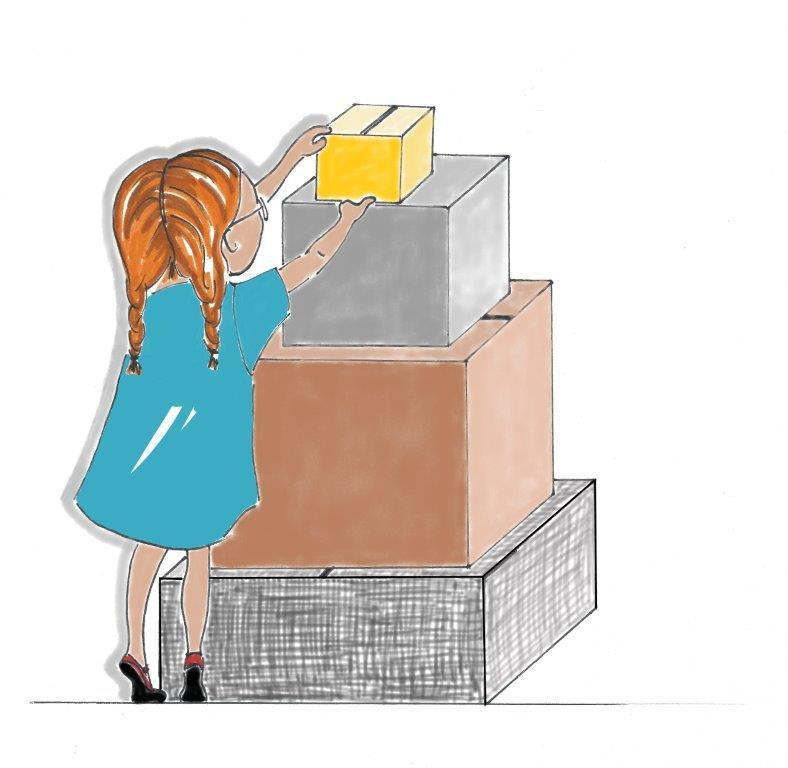
\includegraphics[width=0.6\textwidth]{content/3/chapter4/images/11.png}\\
Cippi prepares the packages
\end{center}

Modules are one of the four big features of C++20: concepts, modules, ranges, and coroutines. Modules promise a lot: shorter compile times, macro isolation, abolishing header files, and avoiding ugly workarounds. Before I present the advantages of modules, I want to step back and explain their benefits.

\subsubsubsection{4.2.1\hspace{0.2cm} Why do we need Modules?}



\subsubsubsection{4.2.2\hspace{0.2cm} Advantages}


\subsubsubsection{4.2.3\hspace{0.2cm} A First Example}

\subsubsubsection{4.2.4\hspace{0.2cm} Compilation and Use}


\subsubsubsection{4.2.5\hspace{0.2cm} Export}

\subsubsubsection{4.2.6\hspace{0.2cm} Guidelines for a Module Structure}


\subsubsubsection{4.2.7\hspace{0.2cm} Module Interface Unit and Module Implementation Unit}


\subsubsubsection{4.2.8\hspace{0.2cm} Submodules and Module Partitions}


\subsubsubsection{4.2.9\hspace{0.2cm} Templates in Modules}


\subsubsubsection{4.2.10\hspace{0.2cm} Module Linkage}


\subsubsubsection{4.2.11\hspace{0.2cm} Header Units}









